\chapter{Results}
\section{Data collection}

Figure \ref{fig:misalignment} visualizes an example of the data collection.
It is observed that the grid by which digits were separated is misaligned with the grid
in which the digits were written. The black grid becomes part of the digit data.
\begin{figure}[H]
\centering
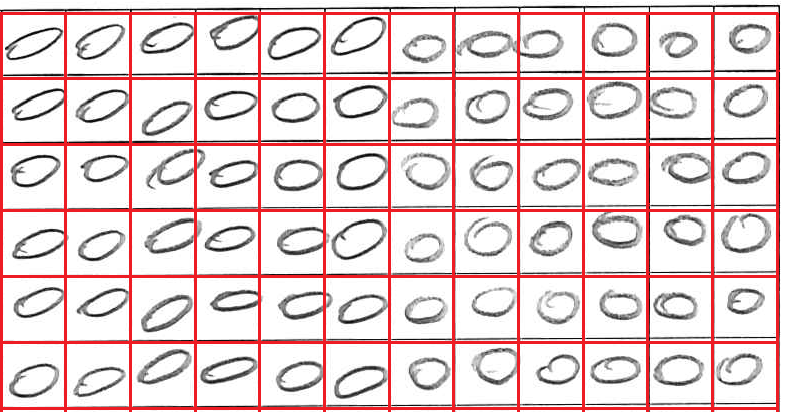
\includegraphics[width  =\textwidth]{figure/kiddi-01-grid-nosmooth-300dpi_cut.png}
\caption{Collected digits. The red grid imposed on the image shows how hand written digits were separated.}
\label{fig:misalignment}
\end{figure}

\section{kNN}
The kNN data processing consists of analyzing the effects of k, smoothing and
DPI density on the error rate  This is found by applying kNN on different training set,
with different smoothing levels, and DPI.

Two smoothing techniques were applied to the images: The average filter, and Gaussian blur.  
For each technique, kNN was applied with different values of k, for which the error rate was calculated.
This allows insight necessary for choosing an optimal k and smoothing parameters.

%% latex table generated in R 3.2.3 by xtable 1.8-2 package
% 
% confusion * 100
% 100 dpi k  = 15
\begin{tabular}{r|rrrrrrrrrr}
%Actual digit
 & 0 & 1 & 2 & 3 & 4 & 5 & 6 & 7 & 8 & 9 \\ 
  \hline
0 & 0.300 & 0.025 & 0.025 & 0.000 & 0.000 & 0.000 & 7.025 & 0.675 & 1.925 & 0.025 \\ 
  1 & 0.000 & 0.675 & 1.325 & 0.000 & 0.000 & 0.000 & 4.475 & 1.950 & 1.400 & 0.175 \\ 
  2 & 0.000 & 0.000 & 2.825 & 0.000 & 0.000 & 0.000 & 1.450 & 3.100 & 2.625 & 0.000 \\ 
  3 & 0.000 & 0.375 & 0.525 & 0.175 & 0.000 & 0.075 & 2.375 & 4.000 & 2.050 & 0.425 \\ 
  4 & 0.025 & 0.050 & 0.025 & 0.025 & 0.175 & 0.025 & 3.700 & 4.250 & 1.475 & 0.250 \\ 
  5 & 0.025 & 0.400 & 0.175 & 0.000 & 0.000 & 1.275 & 4.625 & 0.875 & 2.275 & 0.350 \\ 
  6 & 0.000 & 0.025 & 0.075 & 0.000 & 0.000 & 0.025 & 7.175 & 2.075 & 0.625 & 0.000 \\ 
  7 & 0.000 & 0.125 & 0.725 & 0.000 & 0.000 & 0.075 & 0.275 & 6.675 & 1.775 & 0.350 \\ 
  8 & 0.000 & 0.025 & 0.075 & 0.000 & 0.000 & 0.050 & 5.450 & 1.450 & 2.775 & 0.175 \\ 
  9 & 0.000 & 1.675 & 0.200 & 0.025 & 0.000 & 0.025 & 2.025 & 2.950 & 2.225 & 0.875 \\ 
\end{tabular}
As table
%\ref{tb:confusion}
shows, misclassification occurs in several instances.
Notably, digits 6, 7 and 8 are very often misclassified compared to other digits.
The parameters for this test were 100 DPI and average filter smoothing with kernel size 15.

\begin{figure}[H]    
	\begin{minipage}[t]{0.30\textwidth}
		\centering
			
\includegraphics[width=0.4\linewidth]{Figure/mikael_8_2_dpi100_k1.png}
			\caption{DPI = 100 , kernel size = 1}
			\label{fig:dpi_100_1}
	\end{minipage}
	\hspace{\fill}	
	\begin{minipage}[t]{0.30\textwidth}
		\centering
			
\includegraphics[width=0.4\linewidth]{Figure/mikael_8_2_dpi100_k3.png}
			\caption{DPI = 100 , kernel size = 3}
			\label{fig:dpi_100_3}
	\end{minipage}
	\hspace{\fill}
	\begin{minipage}[t]{0.30\textwidth}
		\centering
			
\includegraphics[width=0.4\linewidth]{Figure/mikael_8_2_dpi100_k5.png}
			\caption{DPI = 100 , kernel size =5}
			\label{fig:dpi_100_5}
	\end{minipage}
\vspace*{0.5cm} % (or whatever vertical separation you prefer)	
	\begin{minipage}[t]{0.30\textwidth}
		\centering
			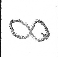
\includegraphics[width=0.4\linewidth]{Figure/mikael_8_2_dpi300_k1.png}
			\caption{DPI = 300 , kernel size = 1}
			\label{fig:dpi_300_5}
	\end{minipage}
\hspace{\fill}	
	\begin{minipage}[t]{0.30\textwidth}
		\centering
			
\includegraphics[width=0.4\linewidth]{Figure/mikael_8_2_dpi300_k5.png}
			\caption{DPI = 300 , kernel size = 5}
			\label{fig:dpi_300_9}
	\end{minipage}	
\hspace{\fill}	
	\begin{minipage}[t]{0.30\textwidth}
		\centering
			
\includegraphics[width=0.4\linewidth]{Figure/mikael_8_2_dpi300_k9.png}
			\caption{DPI = 300 , kernel size = 9}
			\label{fig:dpi_300_9}
	\end{minipage}	
\caption{Effect of smoothing using average filter with different kernel sizes}
\label{fig:average_filter}
\end{figure}

It can be seen based on figure \ref{fig:average_filter} that the smoothing
 filter does have an impact on how clear the digit can be visually
 recognized, and that the higher the DPI density,
  the better visual information. 

Using different smoothing parameters and k, kNN was applied,
using data from one student as training data, and data from another student as testing data.
The correct classification rate was calculated.

\begin{figure}[H]
	\centering
		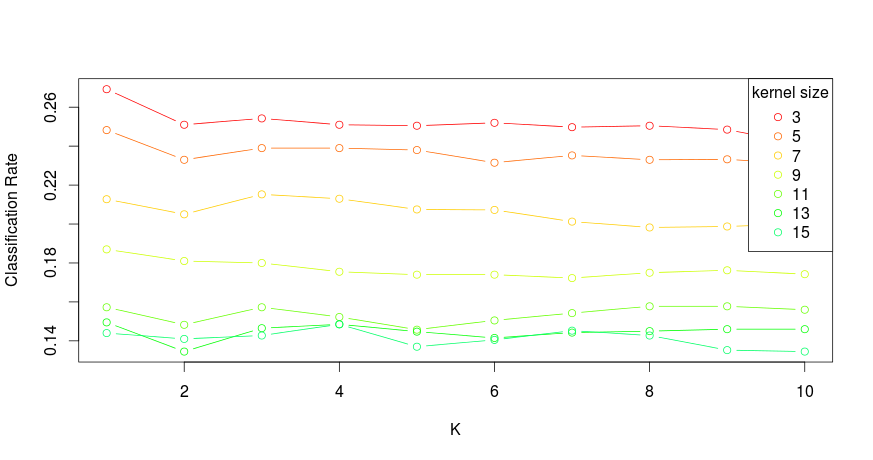
\includegraphics[width = \textwidth]{Figure/data_100_15_10.png}
		\caption{Tested on images with 100 dpi}
		\label{fig:data_100}
\end{figure}

\begin{figure}[H]
	\centering	
		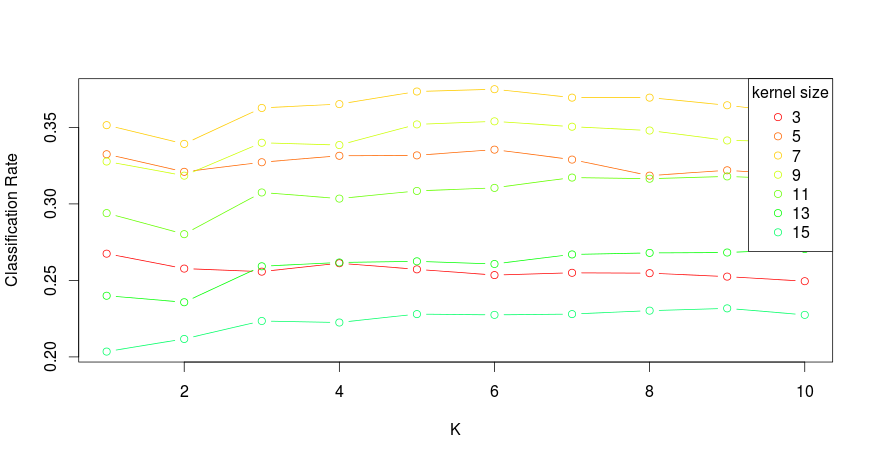
\includegraphics[width = \textwidth]{Figure/data_200_15_10.png}
		\caption{Tested on images with 200 dpi}
		\label{fig:data_200}
\end{figure}

\begin{figure}[H]
	\centering
		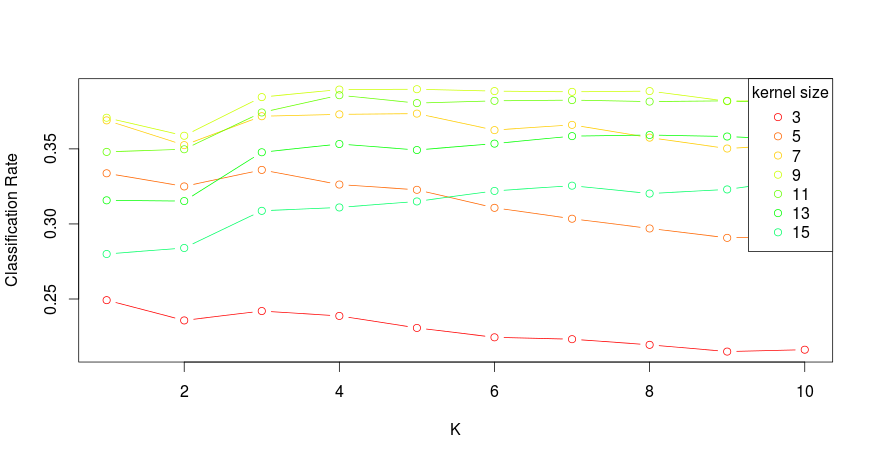
\includegraphics[width = \textwidth]{Figure/data_300_15_10.png}
		\caption{Tested on images with 300 dpi}
		\label{fig:data_300}
\end{figure}

The graphs in figure \ref{fig:data_100} , \ref{fig:data_200}  and \ref{fig:data_300} 
 shows that the images scanned with 300 DPI gives the highest classification rate,
which as previously stated was seen as the ones who gave clearer images as smoothing were applied.
 The graphs shows that the correct classification rate peaks for 100 DPI when applying a kernel at size 3,
 for 200 DPI peaks it is at kernel size 7, and for 300 DPI it peaks at kernel size 9,
 The best perfomance can be found from the images scanned with 300 DPI.
However, very long running times were observed.

\begin{figure}[H]    
	\begin{minipage}[t]{0.30\textwidth}
			\centering
			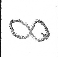
\includegraphics[width=0.4\linewidth]{Figure/mikael_8_2_dpi300_k15_sig_01.png}
			\caption{kernelsize = 15 $\sigma$ = 0.1}
			\label{fig:dpi_300_k_9_s_0.1}
	\end{minipage}
	\hspace{\fill}	
	\begin{minipage}[t]{0.30\textwidth}
		\centering
			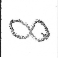
\includegraphics[width=0.4\linewidth]{Figure/mikael_8_2_dpi300_k15_sig_04.png}
			\caption{kernelsize = 15 $\sigma$ = 0.4}
			\label{fig:dpi_300_k_9_s_0.4}
	\end{minipage}
	\hspace{\fill}
	\begin{minipage}[t]{0.30\textwidth}
		\centering
			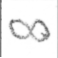
\includegraphics[width=0.4\linewidth]{Figure/mikael_8_2_dpi300_k15_sig_07.png}
			\caption{kernelsize = 15 $\sigma$ = 0.7}
			\label{fig:fig:dpi_300_k_9_s_0.7}
	\end{minipage}
\caption{Effect of smoothing using gaussian filter with different \(\sigma\) values.}
\label{fig:gaussian_filter}
\end{figure}

As an alternative to the average filter could an gaussian filter be used as shown
 in figure \ref{fig:gaussian_filter}. 
Compared to figure \ref{fig:average_filter}, this filter introduces less noise,
and distributes pixel grayscale values more naturally.

